% Compile with XeLaTeX or LuaLaTeX, twice for cross-references.
% Change 169 to 43 here for a traditional 4:3 canvas.
\providecommand{\BeamerAspectRatio}{169}
\documentclass[aspectratio=\BeamerAspectRatio]{beamer}
\usetheme{LeipzigClean}
% Replace these fields for each presentation.
\title[Short title]{Presentation title}
\subtitle{A short subtitle}
\author{First name Last name}
\institute{Department or research group}
\date{Event, Date}
\titlegraphic{}
% Optional link beneath the title metadata:
% \titlegraphic{\small\color{Muted}\href{https://example.org}{Project website}}

\usepackage[backend=bibtex,style=authoryear,maxcitenames=2,maxbibnames=9,natbib=true,doi=true,url=false,isbn=false]{biblatex}
\addbibresource{references.bib}

\begin{document}
\maketitlepage
% Optional overview: uncomment when the talk has multiple sections.
% \maketableofcontents
% Optional section dividers: comment out the next line to hide them.
\makesectionpopup

\section{Example layouts}

% EXAMPLE 1: Short text slide with a single highlighted takeaway.
\begin{frame}{A clear research question}
  \begin{itemize}
    \setlength{\itemsep}{4mm}
    \item Introduce the problem and the audience's reason to care.
    \item State the question in one sentence.
    \item Explain which evidence could answer it.
  \end{itemize}
  \vspace{4mm}
  \keyidea{One main idea per slide}
  \note{Use this space for speaking notes, transitions, or details that do not belong on the slide.}
\end{frame}

% EXAMPLE 2: Text and an image, preserving the image's proportions.
\begin{frame}{Text and figure}
  \begin{columns}[T,onlytextwidth]
    \column{0.53\textwidth}
      \begin{block}{Polarization states}
        The Poincar\'e sphere represents normalized states of fully polarized light.
      \end{block}
      \begin{itemize}
        \item Linear states lie on the equator.
        \item Circular states lie at the poles.
      \end{itemize}
      \vspace{3mm}
      Intensity is a separate quantity.
    \column{0.43\textwidth}
      \centering
      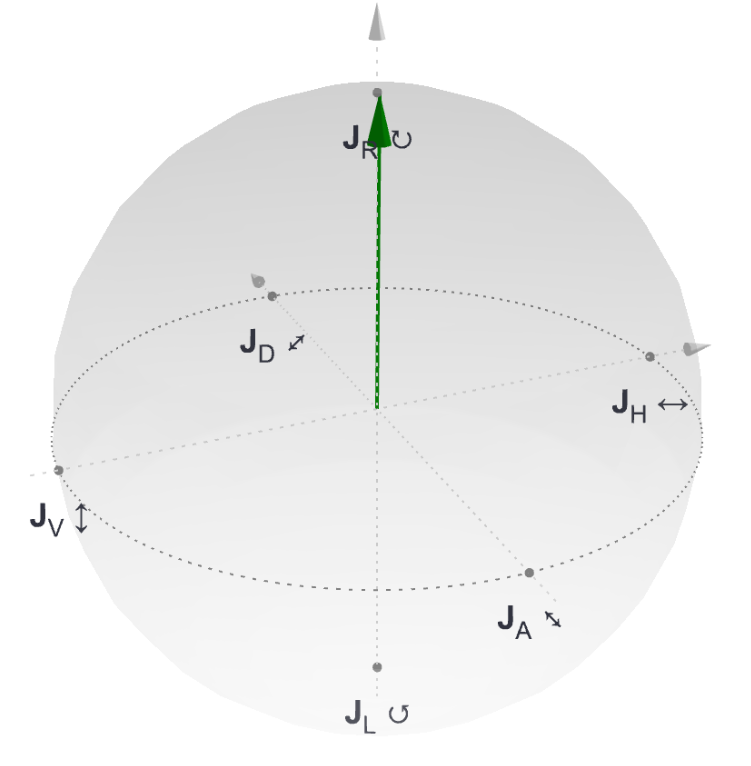
\includegraphics[width=\linewidth,height=.57\textheight,keepaspectratio]{images/poincare.png}
      \source{Example image from the original presentation.}
  \end{columns}
  \slidesource{Source presentation: polarization applet}
\end{frame}

% EXAMPLE 3: Display mathematics and a plain Beamer block.
\begin{frame}{Equations and definitions}
  A normalized Jones vector for a fully polarized state is
  \[
    \mathbf{J}=\begin{pmatrix}a\\b\,e^{i\varphi}\end{pmatrix},
    \qquad a,b\geq 0,\qquad a^2+b^2=1.
  \]
  \vspace{2mm}
  \begin{block}{Notation}
    The amplitudes $a$ and $b$ describe the two transverse components.
    Their relative phase is $\varphi$.
  \end{block}
  \keyidea{Define symbols close to the equation}
\end{frame}

% EXAMPLE 4: An editable table with automatically wrapping columns.
% This table describes layouts, not study findings or invented data.
\begin{frame}{A concise comparison}
  \begin{tabularx}{\textwidth}{@{}P{.20\textwidth}Y Y@{}}
    \toprule
    \textbf{Layout} & \textbf{Typical use} & \textbf{Content} \\
    \midrule
    Text & Introduce a question & A short argument and a takeaway \\
    Text and figure & Explain a visual representation & A figure beside its interpretation \\
    Equation & Define a model & A formula and its variables \\
    Table & Compare alternatives & Consistent categories in each row \\
    \bottomrule
  \end{tabularx}
  \vspace{3mm}
  \source{Example table. Replace these entries with your own content.}
\end{frame}

% EXAMPLE 5: The two visible callout styles from the source deck.
% Beamer's \note{...} is for speaker notes; mynote is visible on the slide.
\begin{frame}{Notes and important points}
  \begin{mynote}[Definition]
    Use a blue callout for a short definition or supporting explanation.
  \end{mynote}
  \vspace{3mm}
  \begin{myalert}[Important distinction]
    Use a red callout for a condition, limitation, or distinction that the audience needs to retain.
  \end{myalert}
\end{frame}

% Closing slide: replace the bracketed text with your own details.
\begin{frame}{Discussion}
  \vfill
  {\Large\bfseries Your main conclusion goes here.\par}
  \vspace{7mm}
  Which question should the audience discuss next?\par
  \vspace{7mm}
  {\small\color{Muted}[Your name]\quad [Your contact or project link]\par}
  \vfill
  Example citation \citep{10.3389/fpsyg.2019.03087}
\end{frame}

\begin{frame}[allowframebreaks]{References}
\renewcommand*{\bibfont}{\scriptsize}
\printbibliography
\end{frame}

% Optional appendix. Disable divider pages for backup material.
% \appendix
% \AtBeginSection[]{}
% \begin{frame}{Additional details}
%   Supporting material goes here.
% \end{frame}

\end{document}
